\chapter{72neV parxkaraNa}

\begin{center}
{\bf\large mUla kamaRvu.}
\vskip .3cm

{\bf mUla kamaRveMdare, vagaR GanAdi mUlagaLanunx tegiyava riVtiyu.}
\vskip .2cm

{\rm  SQUARE ROOT.}
\vskip .3cm

{\bf vagaR mUlavanunx kuritadudx.}
\vskip .3cm

{\bf\large sUtarx.}
\end{center}

\begin{verse}
kaM|| modalaMki viDidumANaRda | tadupariyoMdaMki biTuTx vaMdarameVlaM||
dodagise biMduva padaga | LatxdanaMtara daMshaveraDakUkxMdoMdupadaM||

modalanepadakaM mUlava | nodagisutadarogaRkaLadu matotxdupadaM|| vadagisi sheVSakanaMtara | modalina mUlAMki divxguNagANiseBajakaM||

baMdihaBajakadi BAgisu| taMdAgalubaMda BAgadaMkigaLanUnx|| hiMdina Bajakadi baradada| baMdiha BAgAMkiyiMda guNisuta kaLiyeY||

niMtiha sheVSadamuMda | kekxMtiha matotxMdupadava bariyatameVlina|| aMtara naDigaDi mADuta | leMtAguvadogaR mUla saMKayxvapeVLeY||

vi|| vagARMkigaLalilxruva pUNARMkiya modalaneV aMkiya meVle. hiVge gutuR mADi A meVle baMdaMkiyanunx biTuTx matotxMdaMkiya meVle hAgeV gutuRgaLanunx mADabeVku. yAkaMdare, adariMda pUNARMkigaLu iSuTx padagaLAdaveMtalU padagaLige oMdoMdaMkiya parxkArakekx mUlAMkigaLiSuTx barutatxveyeMtalU gotAtxgutatxve. AdadxriMda hAge padagaLanunx viMgaDisikoMDu, muMde dashAMshagaLalilx eraDeraDaMkigaLige oMdoMdu padadaMteV gotutx mADikoLaLx beVku.
\end{verse}

\begin{enumerate}[\rm (1)]
\item pUNARMkiya modalaneV padada mUlavanunx tegadu adanunx vagARMkigaLa balagaDeyalilx BAgAkAradoVpAdi baradukoMDu. adara vagaRvanunx modalaneV padadalilx kaLadu muMde matotxMdu padavanunx baradukoMDu A meVle modalu baMda mUlAMkiya divxguNavanunx eDagaDege baradukoMDare adu hosa BajakavAgutatxde.

\item A BajakadiMda eSuTxveVLe BAga hoVdiVteMbuvadananxritu, A veVLAMkiyanunx mUla sAthxnadalUlx matutx hiMdina Bajakada mUMdU saha baradukoMDu A oTuTx Bajakavanunx A veVLAMkiyiMda guNisi kaLadu sheVSada muMde matotxMdu padavanunx baradukoMDu, meVlinaMteyeV aduvarige baMda mUlAMkiyanunx divxguNisi eDagaDe baradukoMDu adanunx hosa BajakaveMdu tiLidu adariMda baruva vAyxLAMkiyanunx mUla sAthxnadalUlx matutx adara muMdU saha baradukoMDu A veVLAMkiyiMda punaH Bajakavanunx guNisi kaLiyutAtx sheVSada muMde inonxMdu padavanunx baradukoLuLxtAtx punaH punaH meVlinaMteyeV mADutAtx vagARMkigaLelAlx mugiyuva varigU mADa beVku. Adare bariV dashamAMsha aMkigaLige vagaR mUlavanunx kaMDu hiDiyuvAga dashamAMsha cukekxge aceyiruva yaraDaMkigaLige oMdu padakAkxgiyU muMde eraDeraDaMkigaLige oMdoMdu padagaLanAnxgiyU viSamAMki niMta pakaSxdalilx adakekx sonenxyanunx sheVrisikoMDu padavanunx pUtiR mADikoMDu mUlavanunx kANa beVku.
\end{enumerate}

udAharaNe, $27.5625$ idara vagaR mUlaveSuTx?\\

\begin{tabular}{c>{$}l<{$}>{$}c<{$}}
& 2\dot7.5625 & (525\\
& 25 \\
\cline{2-2}
labadhx $5$ra divxguNa $102$ & \!\!)~ .256\\
& \quad\!204\\
\cline{2-2}
labadhx $52$ra divxguNa $1045$ & )~~~5225\\
& \quad~~\!5225\\
\cline{2-2}
& \quad~~\!0000
\end{tabular}\\

idaralilx pUNARMkiya modalaneV aMki $\dot7$ra meVle cinehxyanunx mADirutatxde A meVle $2$nunx biTuTx muMde aMkigaLiruvadilAlx, AdadxriMda pUNARMkadalilx $27$ oMdu padaveMtalU muMde A pUNARMkiya aMshadalilx $56$ oMdu padaveMtalU $25$ oMdu padaveMtalU gotAtxyitu. Aga modalaneV pada $27$ra mUlavu $5$ AdadxriMda adanunx mUla sAthxnadalilx barakoMDu adara vagaRvAda $25$nunx modalaneV padadalilx kaLiyalU sheVSavu $2$ uLiVtu. adara muMde eraDaneV padavAda $56$nunx baradukoLaLxlu $256$ Ayitu.

Iga modalina mUlavAda $5$nunx divxguNisi Aguva $10$nunx eDagaDige baradukoMDu adariMda sheVSada $25$kekx $2$ veVLe BAga hoVgutatxdeMdu kaMDu A yaraDanunx mUla sathxLadalilx bariyalu $52$ matutx Bajaka $10$ra muMde oriyalu $102$ I parxkArakAkxdavu.

Agalu, A mUlAMki $2$riMda $102$nunx guNisalu $204$ idanunx sheVSa padada keLage baradu kaLiyalu $52$ uLiVtu idara muMde matotxMdu padavAda $25$nunx baradukoLaLxlu $5225$ Ayitu.

punaH Iga mUlAMki $52$ ideyaSeTx adanunx divxguNa mADalu $104$ idanunx eDagaDeyalilx baradukoMDu adariMda sheVSada $522$kekx $5$ veVLe BAgisutatxdeMdu kaMDu A $5$nunx mUlasAthxnadalilx baradukoLaLxlU $525$ matutx eDagaDe Bajaka $104$ra muMde baradukoLaLxlu $1045$ I parxkArakekx Adavu.

Agalu mUlAMki $5$riMda Bajaka $1045$nunx guNisalu $5225$ idanunx sheVSa padada keLage baradukoMDu kaLiyalU sheVSa uLiyalilalxvU. matutx meVlina padagaLU mugadu hoVdavu, AdadxriMda baMda mUlavu $5.25$ eMdu tiLiya beVku.

vayxvahAri BinanxrAshiya vagaR mUlavanunx tegiyuva riVtiyu.

\newpage

\begin{center}
{\bf\large sUtarx,}
\end{center}

\begin{verse}
($1$neVdu) BinanxrAshigaLige dashamAMsha rUpavanunx koTuTx meVle heVLida parxkArakekx vagaR mUlavanunx tegiya bahudu. athavA,

($2$neVdu) kaM|| iriyuta CeVdAMshagaLa | nasxriyAgayxdamUlagaMDu CeVdadiBAgaM|| saribaMdare mUladoLA | girutipaRMshavanu bAgigANalUmxlaM||

vi|| aMsha CeVdagaLa guNAkArada vagaR mUlavanunx tegadu A mUlavanunx CeVdadiMdalAgali, athavA mUladiMda aMshavanAnxgaliV BAgisu.
\end{verse}

udAharaNeyu, $\tfrac{25}{36}$ idara vagaR mUlaveSuTx?\\[5pt]
$
\left.
\begin{tabular}{>{$}c<{$}>{$}c<{$}>{$}c<{$}l}
25 && 5 & idu aMshada mUlavu\\[-7pt]
$-----$&= & $-----$\\[-7pt]
36 && 6 & idu CeVdada mUlavu
\end{tabular}
\right\}
$
\begin{tabular}{c}
hiVge sariyAgidadxre, hiVgU mAda\\
bahudu.
\end{tabular}\\
 

hAgilalxda pakaSxdalilx $25\times36=\sqrt{900}$ idara vagaR mUlavu $30$ Ayitu. Aga $30$ I mUlavanunx CeVdavAda $36$riMda BAgisalu $\tfrac{30}{36}=\tfrac{5}{6}$ mUlavu. athavA mUlavu $30$ idariMda aMsha $25$nunx BAgisalu $\tfrac{25}{30}=\tfrac{5}{6}$idu mUlavu.
udAharaNe, $37542.035$ idara vagaR mUlaveSuTx? \\

$
\left.
\begin{tabular}{l>{$}l<{$}>{$}l<{$}>{$}l<{$}>{$}l<{$}}
&&& \dot37\dot54\dot2.0350 & (193.75\\
&&&1\\
\cline{3-4}
mUlada divxguNa & 29 & )& 275\\
&&& 261\\
\cline{3-4}
mUlada divxguNa & 383 & ) & .1442\\
&&& \;1149\\
\cline{3-4}
mUlada divxguNa & 3867 & )&\quad .29303\\
&&& \quad\;27069\\
\cline{3-4}
mUlada duvxguNa & 38745 & )&\quad\quad223450\\
&&&\quad\quad 193725\\
\cline{3-4}
labadhxda divxguNa & 38750 & )& \quad\quad.29725 & \text{sheVSavu.}\\
\cline{3-4}
\end{tabular}
\right\}
$
\begin{tabular}{>{$}c<{$}}
.10=.1\\
.0001=.01\\
.000001=.001\\
\text{itAyx mUlagaLa}\\
\text{nunx daqSiTxyaninxTiTxra}\\
\text{beVku.}
\end{tabular}\\

I parxkArakekx mUladalilx dashAMsha sathxLagaLu $2$ athavA $3$ baruvavarige mADidAgUyx sheVSa uLadare, A uLida sheVSavanunx BAjayxveMtalU aduvarige baMda mUlAMkiya divxguNavanunx BajakaveMtalU tiLadu dashAMsha saMkeSxVpa BAgAkArada riVtiyiMda BAgisidare, baruva BAga labadhxgaLeV mUlada muMde labadhxvAga beVkAgiruva dashamAMshada aMkigaLAgutatxve. hAyxgeMdare,

meVlina leKaKxdalilx uLida sheVSavu $29725$ idu BAjayxvu. matutx aduvarige baMda mUlada divxguNavu $38750$ idu Bajakavu. Agalu,

\begin{figure}[H]
\centering
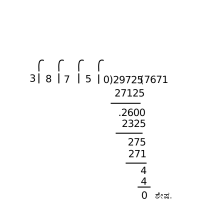
\includegraphics{6.eps}
\end{figure}

I nAlukx aMkigaLanunx mUlaveMdu tiLidu modalina mUlakekx sheVrisikoLaLxlu $193.757671$ idu oTuTx vagaR mUlavu. utatxra.

\begin{center}
{\bf\large 87neV aBayx udAharaNe.}
\end{center}

\begin{tabular}{>{$}l<{$}>{$}l<{$}>{$}l<{$}>{$}l<{$}>{$}l<{$}>{$}l<{$}>{$}l<{$}>{$}l<{$}}
(1) & 17956 & (2) & 55225 & (3) & 2265.76\\[5pt]
(4) & 321489 & (5) & 4596.84 & (6) & 85.5625\\[5pt]
(7) & 4202500 & (8) & 16064064 & (9) & 25401600\\[5pt]
(10)& \tfrac{64}{169} & (11) & \tfrac{25}{49} & (12) & \tfrac{121}{225} & (18) & \tfrac{81}{256}\\[5pt]
(14) & .0005764 & (15) & .000003 & (16) & .000071561\\
\end{tabular}\\

ivugaLanunx $8$ dashAMsha sathxLagaLavarige mUlagaLanunx tegi.
